\section{METHOD}
Figure~\ref{fig:simulation_flow} summarizes the study workflow.
Field records provide two complementary inputs: thermal-preference votes and indoor conditions for fitting PCMs, and room-level entry/exit records that preserve observed attendance and movement as location-log agents.
For each of four target rooms and each sampled subgroup size, PCMs are randomly paired with location-log agents, whose recorded four-week stays are replayed in Monte Carlo trials.
Static, daily, and real-time group comfort models then select setpoints from the same PCM pool at their respective aggregation resolutions.
Person-time comfort probability and the control consequences of real-time updating are evaluated across rooms and sampled group sizes.

\begin{figure}[!htbp]
  \centering
  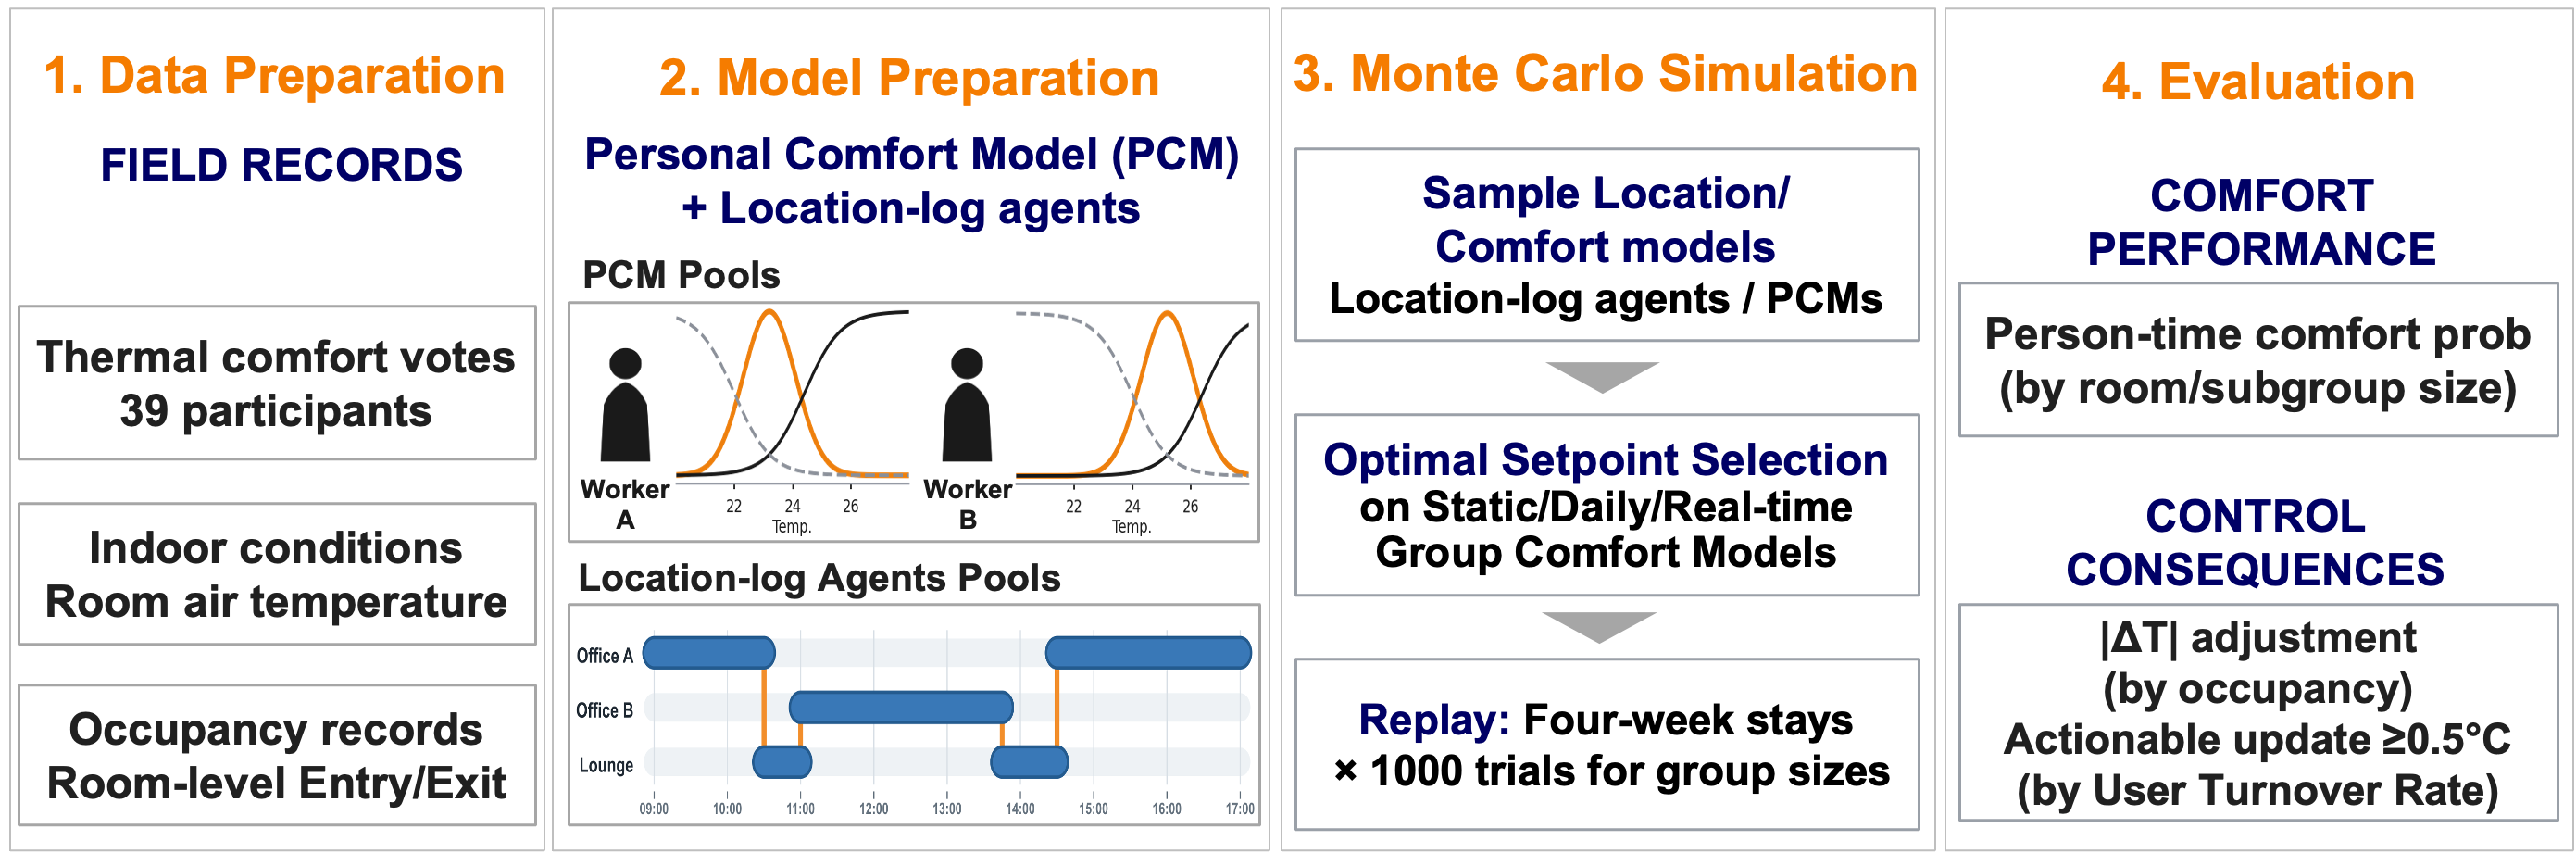
\includegraphics[width=\linewidth]{figures/SimulationFlow_small.png}
  % \includegraphics[width=0.67\linewidth]{figures/SimulationFlow_wider.png}
  \caption{Workflow for the occupancy-log-based Monte Carlo comparison of static, daily, and real-time group comfort models.}
  \label{fig:simulation_flow}
\end{figure}

\subsection{Field data}
Data were collected from 29 September to 24 October 2025 in an office building in Singapore.
The observed rooms were served by a central HVAC system with zone-level VAV control and summarized in~\autoref{table:RoomList}.
\begin{table}[htbp!]
  \centering
  \small
  \caption{Simulation target rooms}
  \begin{tabular}{@{}
    p{2.6cm}
    p{3.8cm}
    M{2.2cm}
    M{1.8cm}
    M{1.8cm}
    @{}}
    \toprule
    \TableHeader{Room} &
    \TableHeaderBreak{Occupants' \TableHeaderLineBreak Job function} &
    \TableHeaderBreak{Seating type} &
    \TableHeaderBreak{Floor area\TableHeaderLineBreak \((\mathrm{m^2})\)} &
    \TableHeaderBreak{Seating\TableHeaderLineBreak capacity} \\
    \midrule
    Office 5A & Real estate development & Assigned & 221.40 & 15 \\
    Office 5B & Research \& development & Assigned & 163.56 & 18 \\
    Shared Office 5A & Real estate development & Shared & 221.40 & 14 \\
    Shared Office 5B & Building construction   & Shared & 213.73 & 20 \\
    \bottomrule
\end{tabular}
  \label{table:RoomList}
\end{table}
Data from 39 participants with sufficiently complete survey records, together with location records for regular room users, were retained.
The protocol was approved by the National University of Singapore Institutional Review Board (NUS-IRB-2025-498) and informed consent was obtained.
Thermal-preference votes were collected by web survey up to six times per workday using the three ASHRAE Thermal Preference categories ``warmer'', ``no change'', and ``cooler'' \parencite{ashrae_ansiashrae_2022}.
Responses within 20 minutes of room entry were excluded to reduce transient exposure effects.
In total, 2,608 responses were available.
Room air temperature and relative humidity were measured while setpoints were varied between 22$^\circ$C and 27$^\circ$C to expose participants to an informative range of conditions.
Anonymized location records were obtained from a face-recognition system installed at room entrances and in corridors and reconstructed into continuous room stays with entry and exit times.

\subsection{Personal and group comfort models}
An ordered multinomial logistic PCM was fitted for each participant using room air temperature as the predictor and thermal preference as the response, following a prior agent-based control study \parencite{jung_energy_2020}.
Let $p_i(T)$ be the PCM probability that occupant $i$ votes ``No change'' at temperature $T$.
For any represented group $G$, the group comfort curve and selected setpoint were

\begin{equation}
 \bar p_G(T)=\frac{1}{|G|}\sum_{i\in G}p_i(T),
 \qquad
 T_G^*=\operatorname*{arg\,max}_{T\in\mathcal{T}_{\mathrm{set}}}\bar p_G(T),
 \label{eq:gcm}
\end{equation}

where $\mathcal{T}_{\mathrm{set}}$ is the candidate setpoint grid (0.1$^\circ$C resolution).
All GCM policies used the same optimization rule; only the group represented by $G$ changed (Table~\ref{tab:policies}).
% This isolates the value of attendance resolution from the setpoint-selection algorithm.

\begin{table}[!htbp]
  \caption{Compared comfort-representation policies.}
  \label{tab:policies}
  \begin{tabularx}{\linewidth}{>{\raggedright\arraybackslash}p{0.19\linewidth}
                                >{\raggedright\arraybackslash}p{0.27\linewidth}
                                >{\raggedright\arraybackslash}X}
    \toprule
    \textit{Policy} & \textit{Represented group} & \textit{Update interpretation} \\
    \midrule
    Static GCM (SGCM) & Sampled regular room members & One group curve for the study period \\
    Daily GCM (DGCM) & Sampled members attending that day & Attendance-aware curve updated daily \\
    Real-time GCM (RT-GCM) & Sampled members present at the interval & Composition-aware curve updated during the day \\
    Baseline & None & Fixed 24$^\circ$C setpoint \\
    \bottomrule
  \end{tabularx}
\end{table}

\subsection{Occupancy-log-based simulation and metrics}
Each trial sampled $K$ location-log agents from a room's regular-member
pool and randomly paired them with $K$ PCMs, randomly drawn without replacement from the pool of 39 PCMs; $K$ denotes the sampled
group size.
The agents retained their observed stay logs in their original rooms; random PCM assignment varied the comfort-profile composition without inventing movement trajectories.
The present set $S_{r,t}$ and instantaneous occupancy $N_{r,t}=|S_{r,t}|$ varied over time.
Decision-time occupancy density was $N_{r,t}/K$; daily mean occupancy $\bar N_d$ was the mean of $N_{r,t}$ over occupied intervals on day $d$, and $\bar N_d/K$ its daily normalized counterpart.
For each room and each feasible $K$, 1,000 trials were simulated over the four-week record.
At every occupied interval, each policy's setpoint was scored against the PCMs of the people actually present.
Mean comfort probability was defined as

\begin{equation}
 \mathrm{CP}_{r,d}^{(\pi,q)}
 =\frac{\displaystyle\sum_{t\in\mathcal{T}_{r,d}}
       \sum_{i\in S_{r,t}^{(q)}}p_i\!\left(T_{r,t}^{(\pi,q)}\right)}
      {\displaystyle\sum_{t\in\mathcal{T}_{r,d}}\left|S_{r,t}^{(q)}\right|}
 % \qquad
 % \overline{\mathrm{CP}}_{r}^{(\pi)}
 % =\frac{1}{Q}\sum_{q=1}^{Q}
 %  \frac{1}{\left|\mathcal{D}_{r}^{(q)}\right|}
 %  \sum_{d\in\mathcal{D}_{r}^{(q)}}\mathrm{CP}_{r,d}^{(\pi,q)}.
 \label{eq:comfort_metric}
\end{equation}

Here, $\pi$ denotes the policy, $q$ the Monte Carlo trial, $\mathcal{T}_{r,d}$ the occupied control intervals for room $r$ on day $d$.
% $\mathcal{D}_{r}^{(q)}$ the valid room-days.
% and $Q=1{,}000$
Room-day values were averaged across days within each trial and then summarized across the 1,000 Monte Carlo trials.
Improvement is reported as a percentage-point difference from the fixed 24$^\circ$C baseline.
Control consequences were summarized by the absolute RT-GCM setpoint change between consecutive intervals and by an actionable-change indicator.
Occupant-composition change was measured using Jaccard turnover.
For a lag $\Delta t$, the occupant turnover rate (UTR) was

\begin{equation}
 \mathrm{UTR}_{r,t}=1-\frac{|S_{r,t}\cap S_{r,t-\Delta t}|}
 {|S_{r,t}\cup S_{r,t-\Delta t}|}.
 \label{eq:utr}
\end{equation}

UTR is zero when the two occupant sets are identical and one when they have no members in common.
The main action-frequency result uses 15-minute transitions.
% A transition was classified as actionable when the setpoint changed by at least 0.5$^\circ$C.